\section{Design}
This section presents the overall design of the Lapsus system and provides a comprehensive overview of the solution’s structure and the interaction between its individual components. The section focuses on the system architecture, key design decisions, and the physical and digital design of the solution.

The design is illustrated through a series of UML and system diagrams, which collectively describe the system’s context, functional relationships, and technical structure. In addition, the design of the wristband, the 3D-printed enclosure, and the mobile application along with its underlying infrastructure are described. The purpose is to clarify how the overall solution is composed and how the various components operate together in practice.

\subsection{Design of the solution}
This section describes the design of the overall Lapsus solution, with a focus on the system’s structure. The design is based on the knowledge and insights obtained through analysis and the state of art section and translates these into a technical solution.

The section introduces the core system components and their relationships and provides the foundation for the subsequent diagrams that illustrate system interactions and architecture. The purpose is to present a clear and structured overview of how the system is constructed.

\subsubsection{Use case diagram}
The use case diagram (see \autoref{fig:use-case-diagram}) highlights the use cases in the system boundary. Here, it is seen that the user can log in through the backend. The user can also add relatives to the database. Furthermore, the user can connect to the wristband through Bluetooth between the wristband and a phone. The user can also cancel the alarm and press the emergency button, which goes through the database and backend. In the system boundary, the relatives can log in and view the \gls{gps} location of the user in real time, both of which use the backend.

\begin{figure} [H]
    \centering
    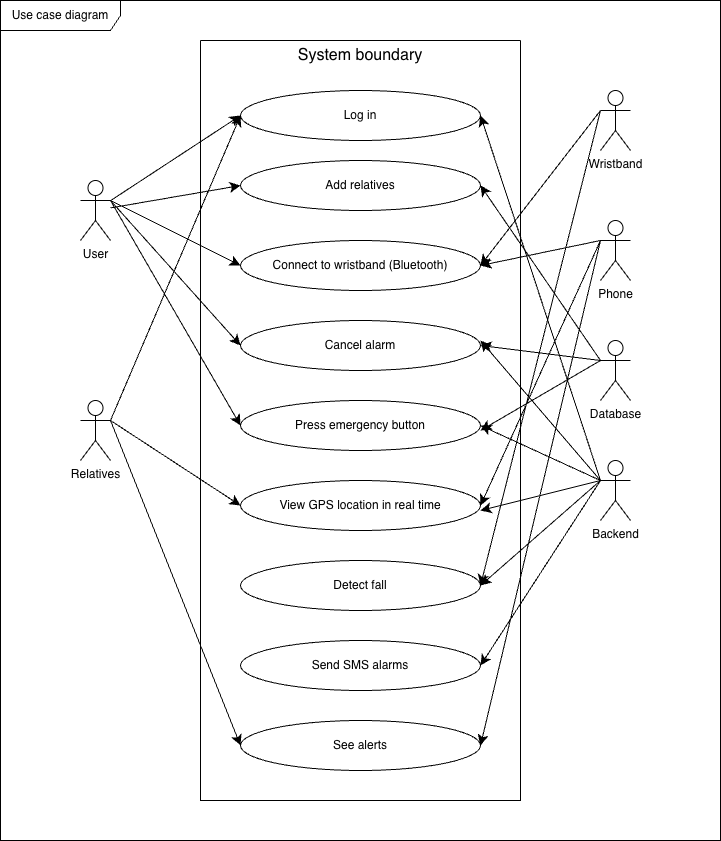
\includegraphics[width=1\linewidth]{report/images/Use case diagram P3.drawio.png}
    \caption{Use case diagram}
    \label{fig:use-case-diagram}
\end{figure}

\subsubsection{Context diagram}
The defined requirements, together with insights from the state of art analysis, form the foundation for the overall system structure of Lapsus. Based on this knowledge, the context diagram was developed to provide a high-level representation of the system and its interaction with external entities. The diagram reflects key design decisions derived from the requirements, including the central role of the mobile application, the exclusion of an internal alarm center, and the reliance on relatives as the primary responders.

The context diagram in \autoref{fig:contextdiagram} gives an overview of the application as a system. Here it is seen that there are four external entities: wristband, user, Firebase and relatives. 
The first dataflow \textit{detect fall} goes from \textit{wristband} to the application. Then, from the user, the data \textit{add relatives} and \textit{cancel alert} flows to the application. From the application, the dataflows \textit{fall detection alert} and \textit{location data} are sent to the relatives. Lastly, the application sends the \textit{add users and relatives}, \textit{location data} and \textit{login request} data to Firebase, where Firebase can send the \textit{list of relatives}, \textit{location history} and \textit{login token (\gls{jwt})} data to the application. 

\begin{figure}[H]
    \centering
    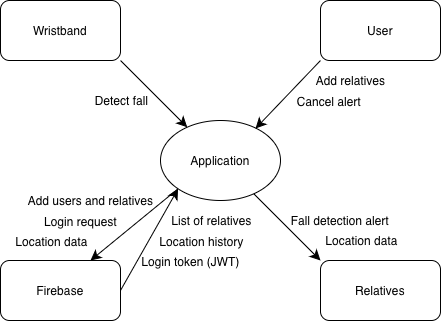
\includegraphics[width=0.75\linewidth]{report//images/Context.drawio.png}
    \caption{Context diagram for the system}
    \label{fig:contextdiagram}
\end{figure}






\subsection{Wristband design}

du kan omskrive krav 17 (detect 90 percent falls) til at have en parentes med senitivity, da det er et begreb Peter nævner i table 2 fra SOTA
\subsection{3D print design}
The physical enclosure of the wristband was designed and prototyped using 3D printing. This approach enabled rapid iteration and made it possible to adapt the design throughout the development process.

The enclosure was designed to securely house the electronic components while keeping the overall dimensions as compact as possible. Particular attention was given to the placement of the emergency button to ensure that it is easily accessible without being prone to accidental activation.

The enclosure consists of two parts: a base that holds the dev board and battery, and a top cover that protects the components while allowing interaction with the button. Openings for charging and ventilation were minimized to improve durability and support future waterproofing considerations.

\begin{figure}[H]
    \centering
    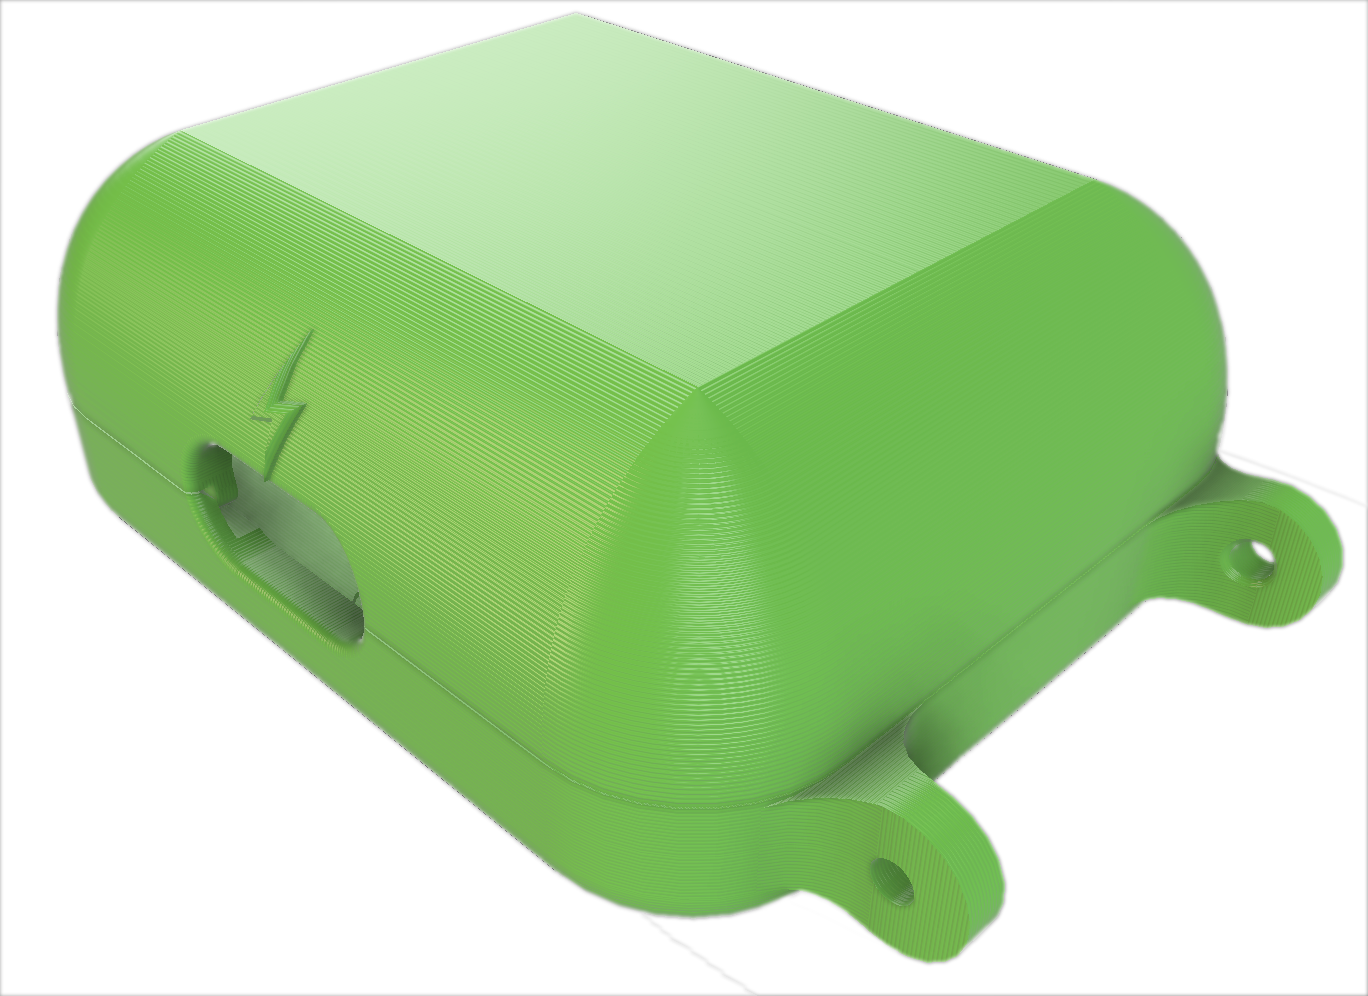
\includegraphics[width=0.5\linewidth]{report//images/Enclosure B.png}
    \caption{Wristband Enclosure}
    \label{fig:wristband_enclosure}
\end{figure}

The use of 3D printing allowed quick adjustments to tolerances and dimensions based on assembly testing. This proved especially valuable when fitting the battery and ensuring sufficient space for wiring and connectors.


\subsection{App design \& solution}

We chose to develop an app with the capacitor framework (citation needed). It allows a single codebase to be compiled into both an iOS and Android app, saving development time and complexity. It works by presenting a website as a native app, and creating api's for the native layers of each of the possible operating systems features, such as cameras, location, contacts etc.

That way, the web app is not limited to the typical restrictions of websites, but still has access to the same features as regular native apps.

\subsubsection{User interface \& user experience}
For a faster and easier time developing, we chose to use a framework for the ui as well. For this we chose the mantine framework (citation needed)  due to its sleek design and many helper utilities.

\subsection{System-functionalities}




\subsubsection{Data flow diagram}
til opdatering af diagram
- øverste dataflow skal hedde phone nr og kode
- realtime skal ændres til real-time
- gps skal ændres all around til GPS
\begin{figure} [H]
    \centering
    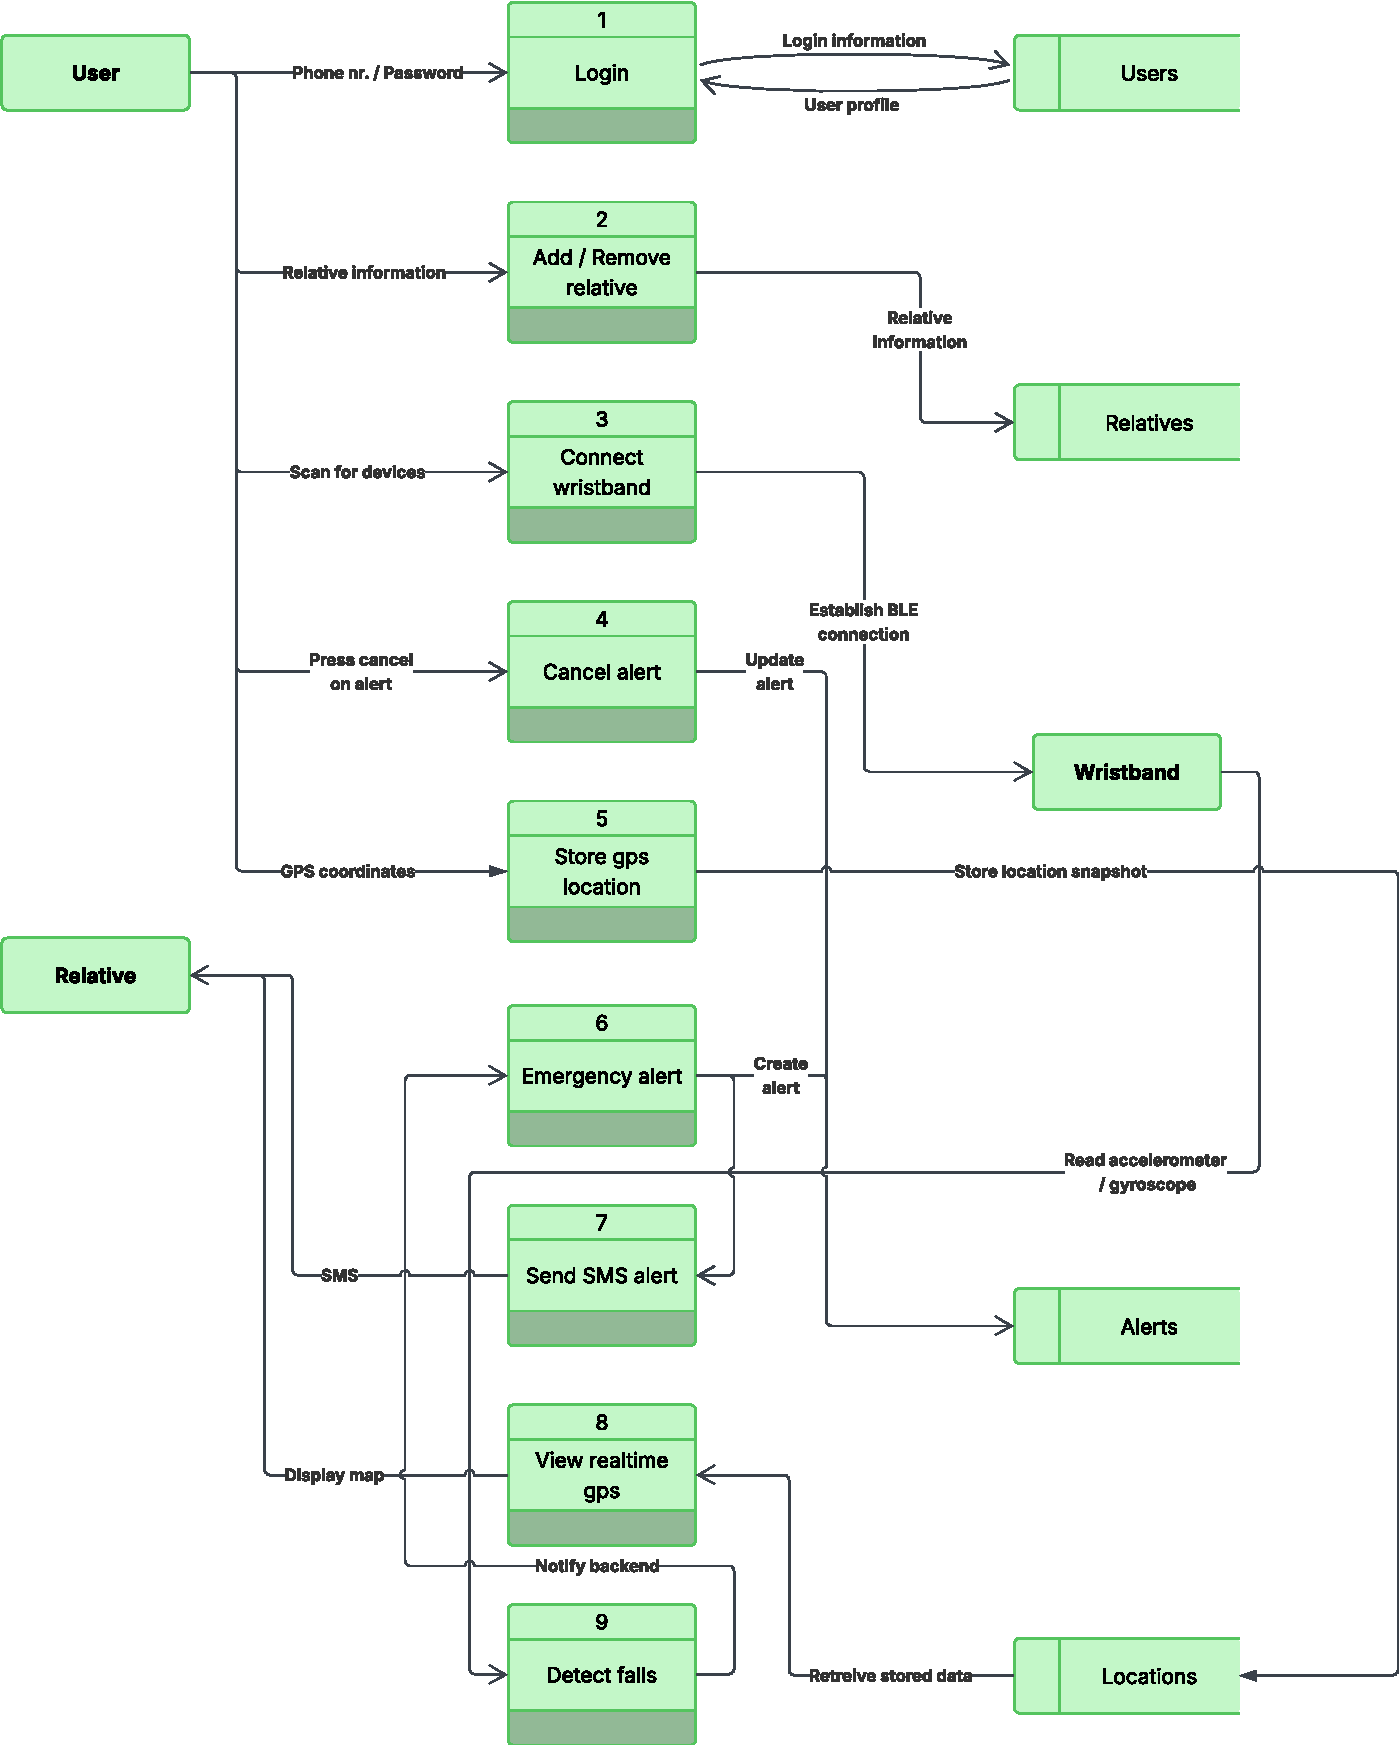
\includegraphics[width=1\linewidth]{Dataflow-Diagram-med-line-jumps.pdf}
    \caption{Data flow diagram over Lapsus}
    \label{fig:placeholder}
\end{figure}

\subsubsection{Sequence diagram}
The sequence diagram below describes the sequence when a fall is detected. The fall is detected by the wristband, which then notifies the mobile app. The mobile app creates the alert, and a new entry is created in the database in the backend. After this, the backend alerts the relative, where they can then respond to the alert. The ‘optional’ shows how a fall can be canceled by the user, in which case the mobile app cancels the alert, and the backend updates the corresponding database entry. After this, the backend notifies the relative, who can then contact the user regarding the canceled alert.  
\begin{figure}[H]
    \centering
    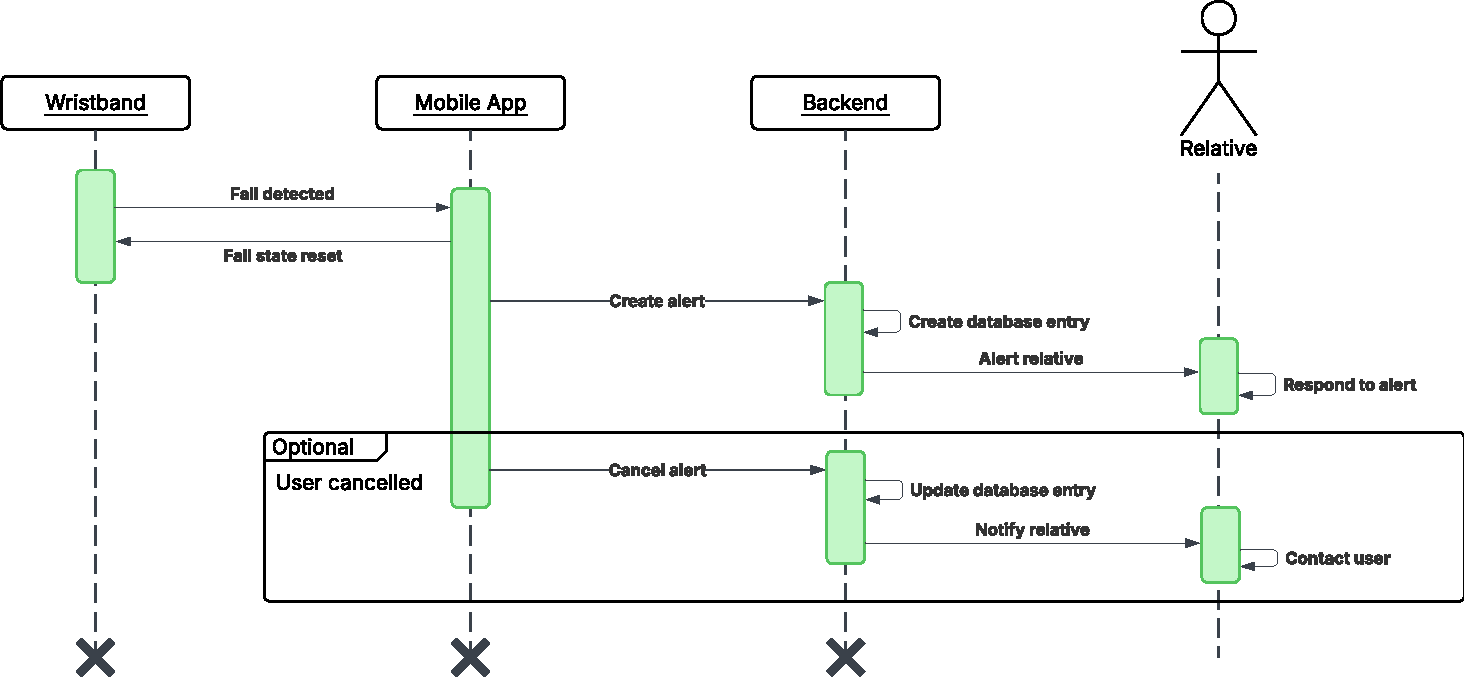
\includegraphics[width=1\linewidth]{Sequence-Diagram-Sequence-Diagram.pdf}
    \caption{Enter Caption}
    \label{fig:placeholder}
\end{figure}

\subsubsection{Deployment diagram}
In the following deployment diagram, 
\begin{figure} [H]
    \centering
    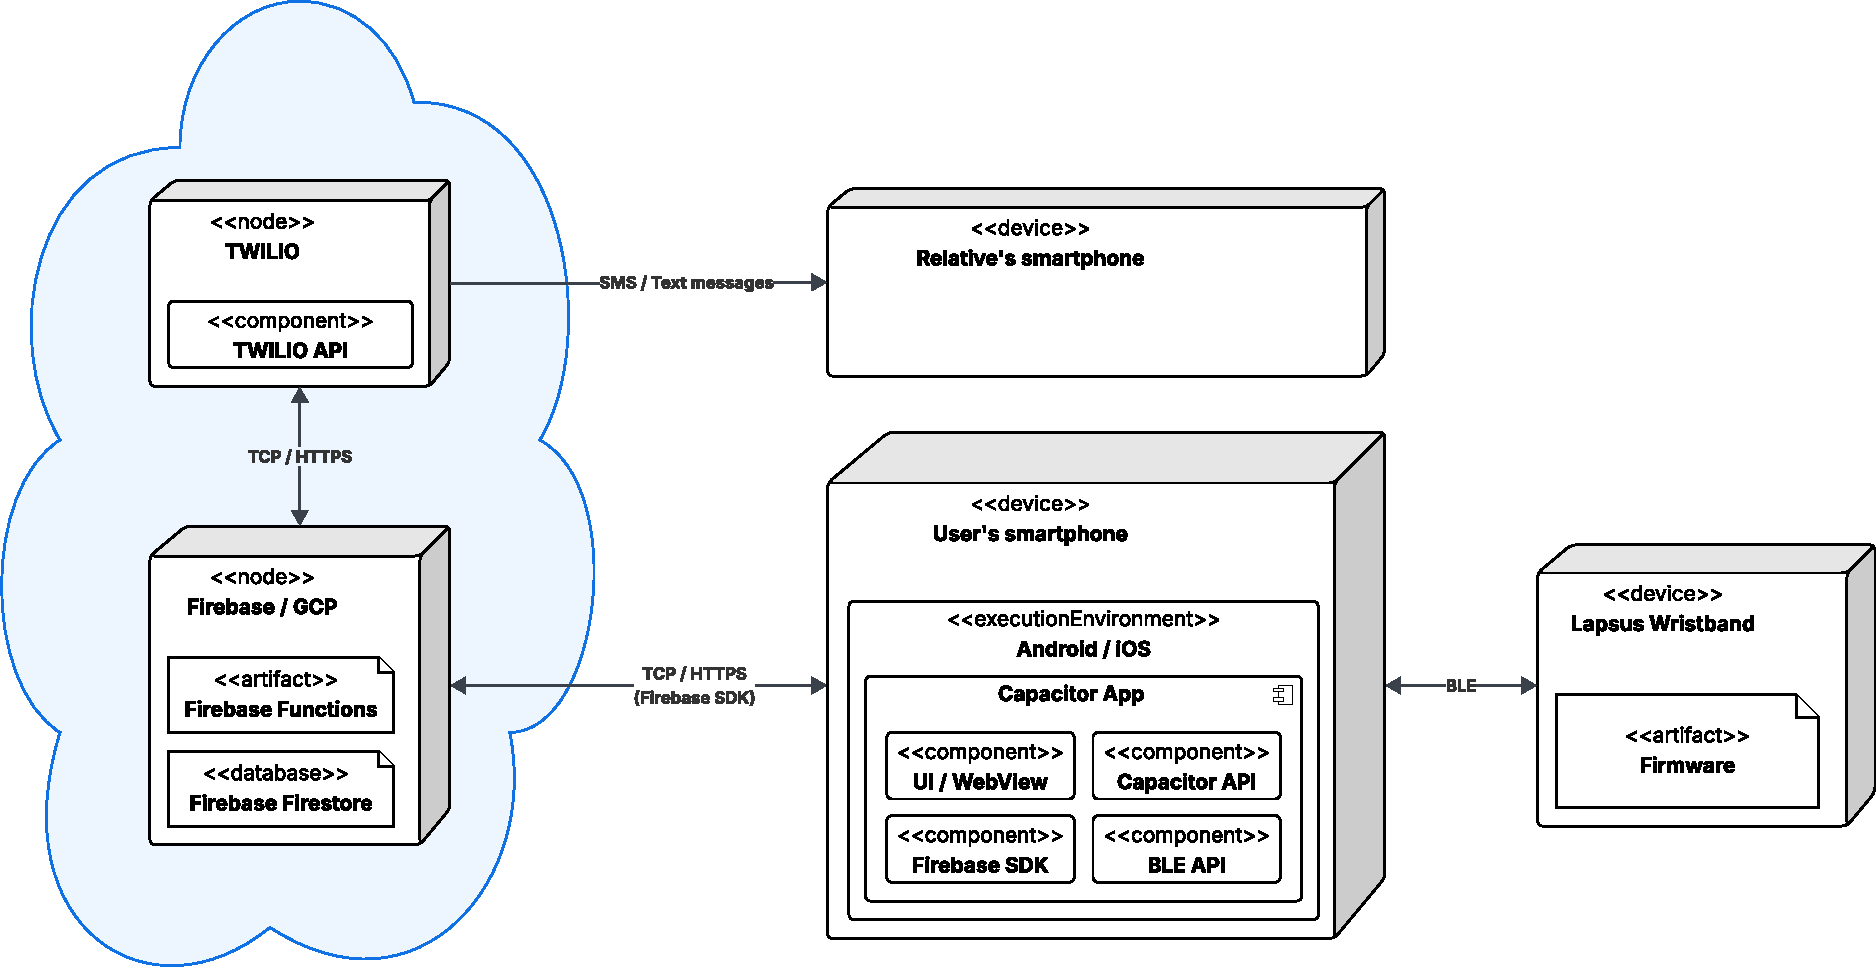
\includegraphics[width=1\linewidth]{Deployment-Diagram-Deployment-Diagram.pdf}
    \caption{Enter Caption}
    \label{fig:placeholder}
\end{figure}

